Zeichnen Sie ein Phasendiagramm f"ur die Differentialgleichung
\begin{equation}
y'=\sin y,
\label{601:dgl}
\end{equation}
finden Sie die kritischen Punkte und bestimmen Sie, welche kritischen
Punkte stabil sind und welche instabil.

\begin{loesung}
Die kritischen Punkte sind die Nullstellen von $\sin y$, also die
Zahlen $k\pi$, $k\in\mathbb Z$.
F"ur $y\in[2k\pi,(2k+1)\pi]$ ist $\sin y$ positiv, in allen
anderen Intervallen ist $\sin y$ negativ.
L"osungen mit Anfangswerten in $[2k\pi,(2k+1)\pi]$ streben daher
gegen $(2k+1)\pi$, solche mit Anfangswerten in $[(2k+1)\pi, (2k+2)\pi]$
streben gegen $(2k+1)\pi$.
Somit sind die geraden Vielfachen von $\pi$ instabile Fixpunkte
und die ungeraden Vielfachen sind stabile Fixpunkte.
\end{loesung}

\begin{diskussion}
Die Differentialgleichung l"asst sich mit Separation l"osen:
\[
\int \frac{dy}{\sin y}
=
\int\,dx
\quad\Rightarrow\quad
\log\frac{\cos y-1}{\cos y+1}
=
2x+C
\quad\Rightarrow\quad
\frac{\cos y-1}{\cos y+1}
=
Ke^{2x}.
\]
Da $\cos y-1\le 0$ und $\cos y +1\ge 0$ gitl, ist der Bruch auf der linken
Seite $\le 0$, und daher muss $K\le 0$ sein.
Wir schreiben daher $L=-K$, $L$ ist jetzt $\ge 0$.
Wir m"ussen den Bruch auf der linken Seite nach $\cos y$ aufl"osen:
\begin{align*}
\cos y - 1 &=-Le^{2x}\cos y -Le^{2x}
\\
\cos y(1+Le^{2x})
&=
1-Le^{2x}
\\
\cos y
&=
\frac{1-Le^{2x}}{1+Le^{2x}}
=
\frac{e^{-x}-Le^{x}}{e^{-x}+Le^x}
\end{align*}
Schreiben wir jetzt $L=e^{2\kappa}$, dann k"onnen wir den letzten
Ausdruck umformen zu
\begin{equation}
\cos y
=
\frac{e^{-x}-e^{2\kappa}e^x}{e^{-x}+e^{2\kappa}e^x}
=
\frac{e^{-\kappa}e^{-x}-e^{\kappa}e^x}{e^{-\kappa}e^{-x}+e^{\kappa}e^x}
=
\frac{e^{-(x+\kappa)}-e^{x+\kappa}}{e^{-(x+\kappa)}+e^{x + \kappa}}
=
-\frac{\sinh(x+\kappa)}{\cosh(x+\kappa)}
=
-\tanh(x+\kappa)
\label{601:cos}
\end{equation}
Damit ist die L"osung
\[
y=\arccos(-\tanh(x+\kappa)).
\]
Weitere L"osungen entstehen aus den zus"atzlichen L"osungen der
Gleichung~(\ref{601:cos}).
Die L"osungen sind in Abbildung~\ref{601:bild} dargestellt.
\begin{figure}
\centering
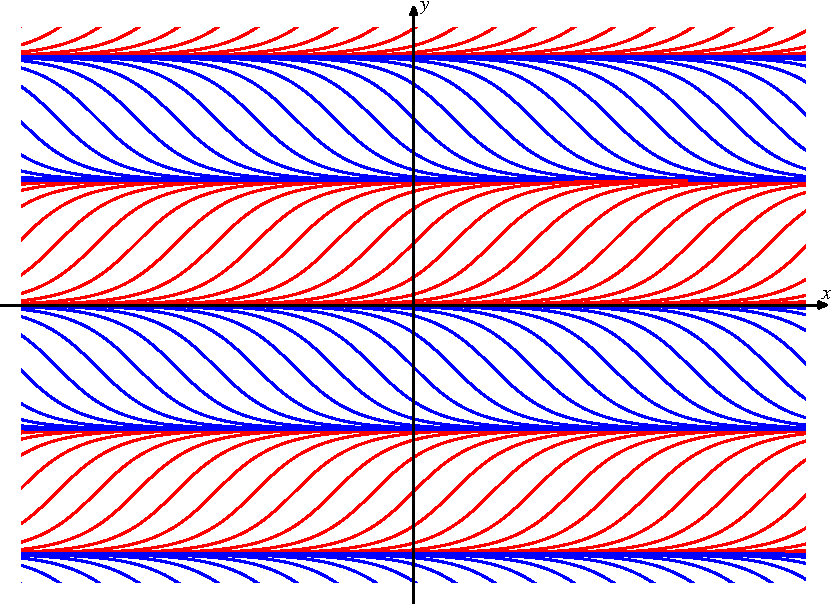
\includegraphics{uebungsaufgaben/601-1.pdf}
\caption{L"osungen der Differentialgleichung~(\ref{601:dgl})
\label{601:bild}}
\end{figure}
\end{diskussion}

